
\begin{enumerate}
    \item In a Young's double slit experiment, the slit separation \(d\) is 0.3 mm and the screen distance \(D\) is 1 m. A parallel beam of light of wavelength 600 nm is incident on the slits at angle \(\alpha\) as shown in figure. On the screen, the point \(O\) is equidistant from the slits and distance \(PO\) is 11.0 mm. Which of the following statement(s) is/are correct?
        \begin{tasks}(2)
            	\task For \(\alpha = \frac{0.36}{\pi}\) degree, there will be destructive interference at point \(O\).
            	\task For \(\alpha = 0\), there will be constructive interference at point \(P\).
            	\task For \(\alpha = \frac{0.36}{\pi}\) degree, there will be destructive interference at point \(P\).
            	\task Fringe spacing depends on \(\alpha\).
        \end{tasks}
\end{enumerate}
\begin{center}
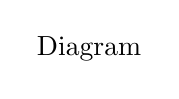
\begin{tikzpicture}
\node {Diagram};
\end{tikzpicture}
\end{center}
